\section{Air Pollution and Particulate Matter}

Air pollution has an impact on the health of communities and individuals, such as cardiovascular and respiratory diseases, strokes and cancers \cite{scor}. According to the World Health Organization (WHO) \cite{whofactsheet}, "more and more, evidence demonstrating the linkages between ambient air pollution and the cardiovascular disease risk is becoming available". Air pollution sources can be anthropological, such as burning fossil fuels, agriculture and waste treatment or they can be natural sources such as volcanic eruptions, forest fires and sand storms \cite{signals}.

Particulate Matter (PM) is a mixture of solid and liquid particles found in the air. Some of them are not visible with the naked eye and are absorbed by our lungs when inhaled. PM is measured in micrograms per cubic meter ($\mu g m^{-3}$) and can have several size filters: $PM_{10}$ which includes particles which are $10\mu m$ or smaller, $PM_{2.5}$ which includes particles which are $2.5\mu m$ or smaller and  $PM_1$ which includes particles smaller than $1\mu m$.

Exposure to PM2.5, in particular, has been studied to have a negative impact on people's health and was attributed the fifth-ranking mortality risk factor in 2015 \cite{lancet}.

The World Health Organization Air Quality Guidelines state that fine particulate matter (PM2.5) should not exceed 10 $\mu g/m^3$ annual mean and 25 $\mu g/m^3$ 24-hour mean and coarse particulate matter (PM10) should not exceed 20 $\mu g/m^3$ annual mean and 50 $\mu g/m^3$ 24-hour mean \cite{whofactsheet}. The same organisation reports that ambient air pollution was estimated to cause 4.2 million premature deaths in 2016 worldwide due to exposure to PM2.5, 91\% of those in low- and middle-income countries, especially in the South-East Asia and Western Pacific regions \cite{whofactsheet}. WHO is deeply committed to responding to the adverse health effects of air pollution. 


\section{AIRSpeck and RESpeck sensors}

The RESpeck sensor (Figure \ref{fig:e}) is a respiratory monitor that includes a 3-axis gyroscope and accelerometer that is worn as a plaster on the chest, as observable in Figure \ref{fig:f}. It allows tracking respiratory movements such as breathing rate and other breathing properties \cite{estimation_dosage}. 

The AIRSpeck family of sensors \cite{airspeck_family} is comprised of two sensors: the AIRSpeck-S (Stationary) and the AIRSpeck-P (Personal), the latter often referred to as mobile sensor in this project, given its wearable usability. The AIRSpeck-S, observable in Figure \ref{fig:b} is a portable stationary sensor that can be attached to street furniture and measure temperature, humidity, $PM_1$, $PM_{2.5}$, $PM_{10}$, nitrogen dioxide ($NO_2$) and ozone ($O_3$) concentrations. The sensor components are listed in Figure \ref{fig:a}. The PM values are derived from an Optical Particle Counter that classifies particles by size between $0.38\mu m$ and $17 \mu m$ into 16 different categorised bins. Data from AIRSpeck-S sensors are sent to a server through the GSM network using a GPRS module. The AIRSpeck-P sensor provides similar functionality in a different form factor (Figure \ref{fig:c}). It includes a battery and can be worn as a belt (Figure \ref{fig:d}) or sash and be used to monitor personal exposure of pedestrians. AIRSpeck-S sensors collect data every 5 minutes, while AIRSpeck-P sensors collect at a higher rate of 10 seconds.

The AIRSpeck family of sensors and RESpeck sensor were developed by the Centre for Speckled Computing at the University of Edinburgh. Both types of sensor communicate via Bluetooth with an Android application that stores the information collected from sensors and other information such as GPS coordinates and device battery levels \cite{clinical_trials}. Their lower cost, when compared to other high-end systems, high accuracy and high-cost sensors, allow an implementation of a network of these sensors for recording higher amounts of data both in space and in time.

The AIRSpeck sensors use Alphasense OPC-N2 sensor for measuring PM concentrations. In the Particle Counter's User Manual \cite{alphasense}, using the European standard definition of $PM_1$ and $PM_{10}$, the sensor assumes "a negligible contribution from particles below (...) the lower limit of particle detection of the OPC-N2 sensor" and "PM10 extends to particle sizes beyond the upper measurable size limit of the OPC-N2. In some cases, this can result in the reported PM10 value being underestimated by up to ~10\%". Given the possibility of $PM_1$ and $PM_{10}$ measurements having less precision than $PM_{2.5}$ in a low pollution environment such as the city of Edinburgh, and the fact that $PM_{2.5}$ has been proven to have a negative impact on people's health, this project focused on $PM_{2.5}$. However, this model can be applied to other PM values and possibly other pollution metrics such as ozone or nitrogen dioxide concentrations.


\begin{figure}[H]
\centering
\begin{subfigure}{0.48\textwidth}
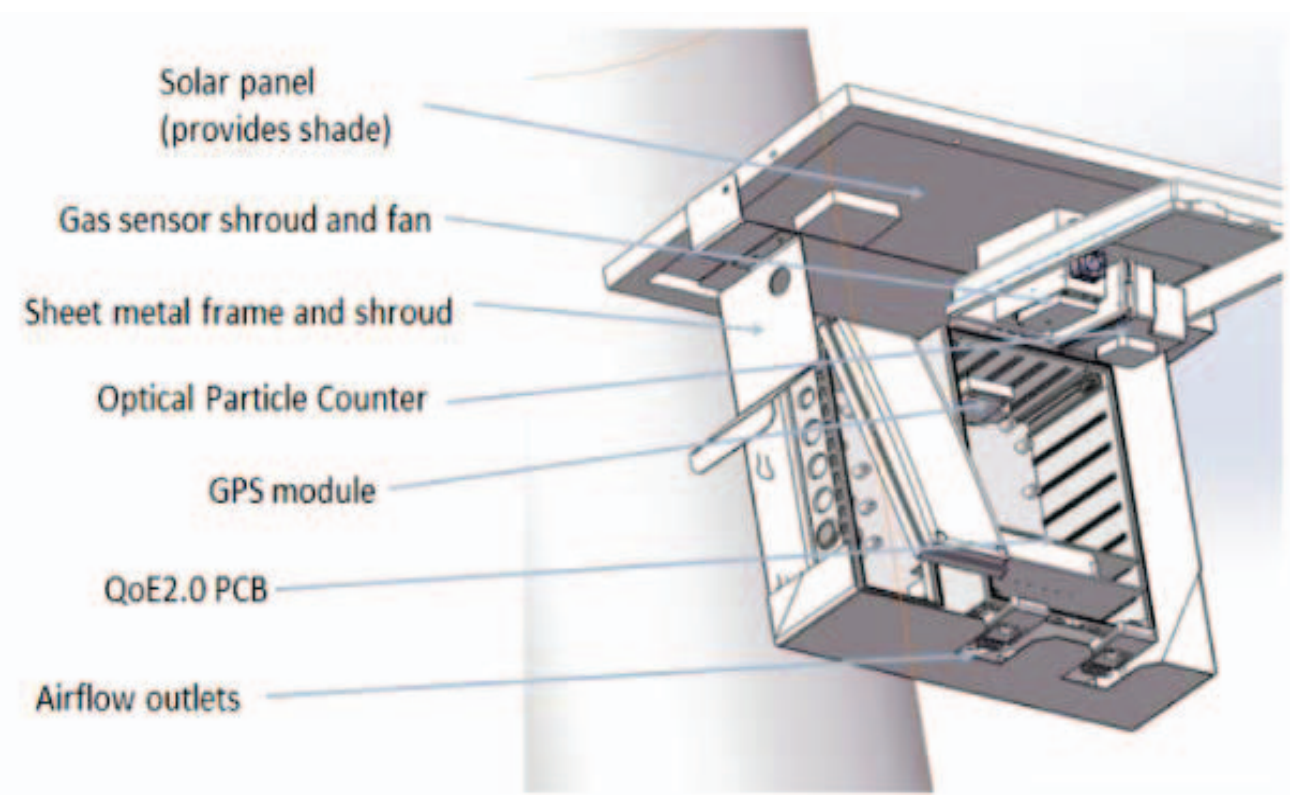
\includegraphics[width=\linewidth]{images/Airspeck_P_inside.png}
\caption{AIRSpeck S composition \cite{clinical_trials}} \label{fig:a}
\end{subfigure}
\begin{subfigure}{0.48\textwidth}
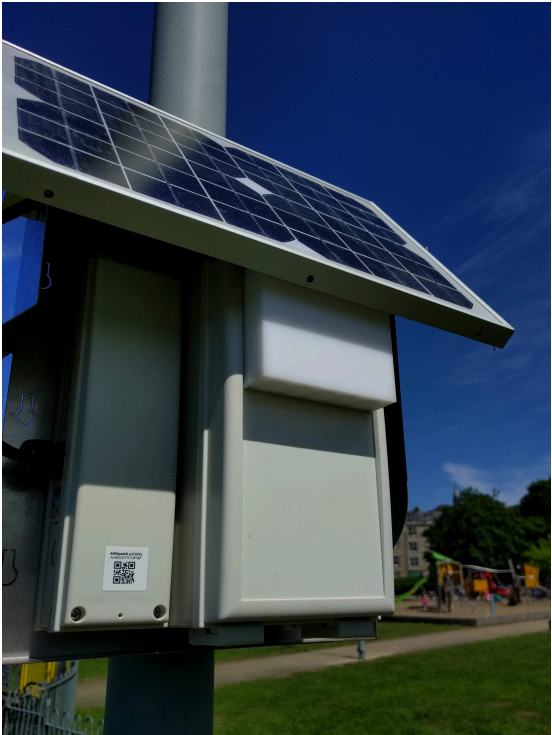
\includegraphics[width=\linewidth]{images/AirspeckS.png}
\caption{AIRspeck S sensor \cite{zoe}} \label{fig:b}
\end{subfigure}

\medskip


\begin{subfigure}{0.48\textwidth}
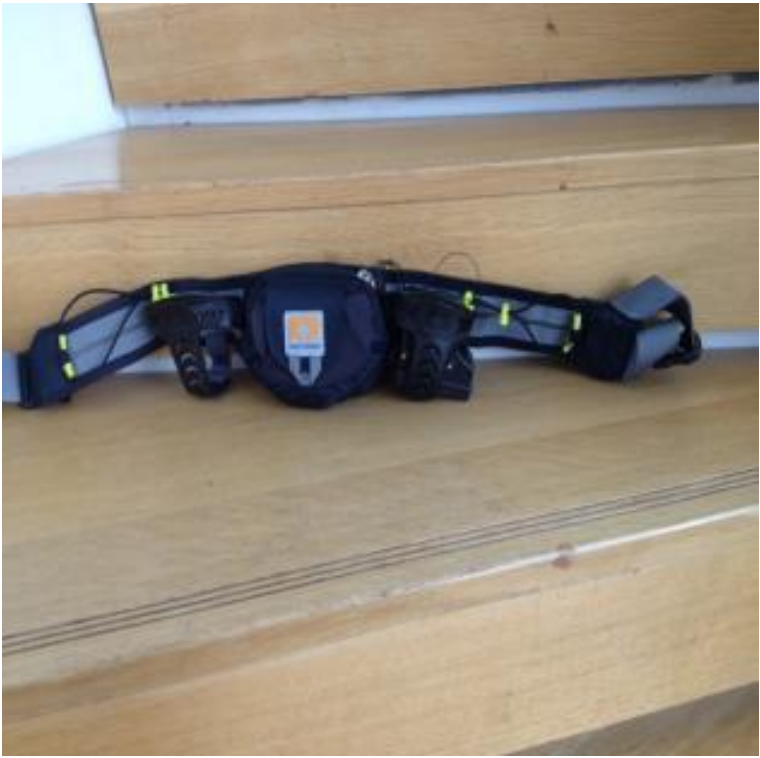
\includegraphics[width=\linewidth]{images/AIRSpeckP.png}
\caption{AIRSpeck P sensor belt \cite{estimation_dosage}} \label{fig:c}
\end{subfigure}
\begin{subfigure}{0.48\textwidth}
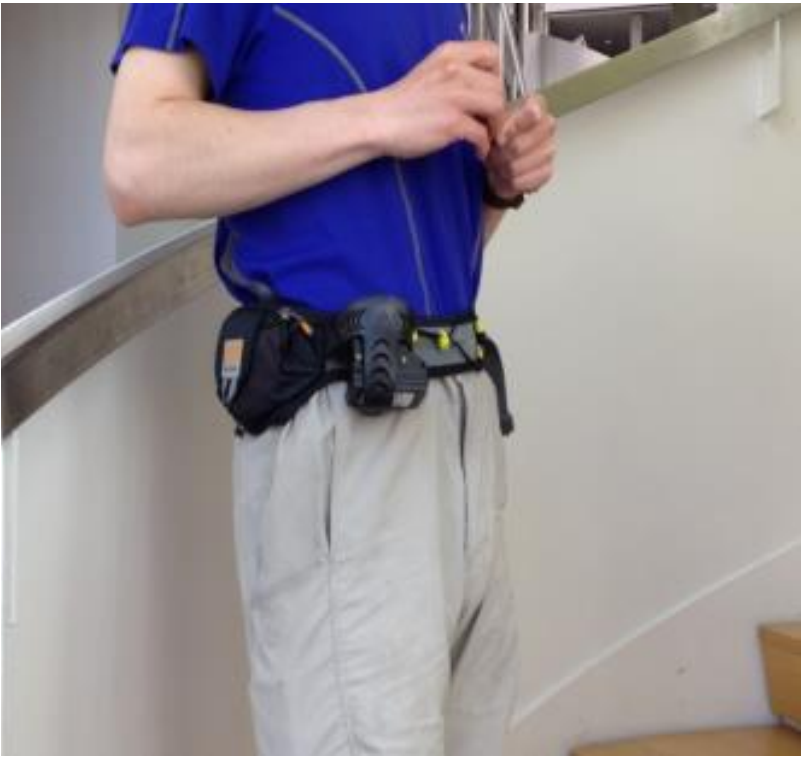
\includegraphics[width=\linewidth]{images/AIRSpeck_P_worn.png}
\caption{AIRSpeck P sensor worn \cite{estimation_dosage}} \label{fig:d}
\end{subfigure}

\medskip

\begin{subfigure}{0.48\textwidth}
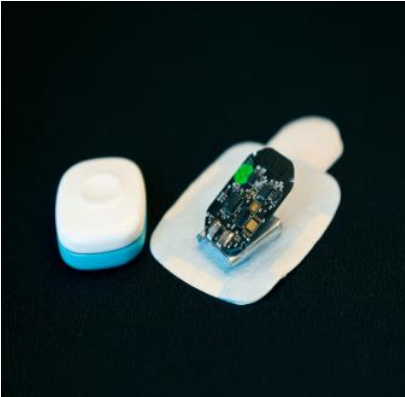
\includegraphics[width=\linewidth]{images/RESpeck.png}
\caption{RESpeck sensor \cite{estimation_dosage}} \label{fig:e}
\end{subfigure}
\begin{subfigure}{0.48\textwidth}
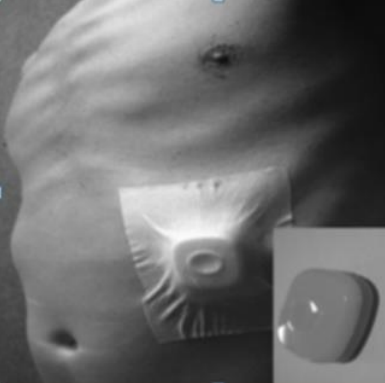
\includegraphics[width=\linewidth]{images/RESpeck_worn.png}
\caption{RESpeck sensor worn on body \cite{estimation_dosage}} \label{fig:f}
\end{subfigure}

\caption{AIRspeck and RESpeck sensors}
\label{fig:sensors}
\end{figure}



\section{Online Machine Learning}
The batch learning method is one of the most commonly used machine learning techniques, also referred to as offline techniques. In batch learning, the best predictor is generated using the entire dataset at once. On the other hand, in online techniques, data becomes available in sequential order and the model updates at each step when data becomes available. Not only an online algorithm makes predictions in real time, but it also trains in real time. This difference in paradigm to "learn" the best predictor can be observed by comparing Figure \ref{fig:batch} and \ref{fig:online}. The online model works in "rounds": at the beginning of each round, an input sample is presented and a prediction is performed. The algorithm verifies if the prediction was good or not and adjust its parameters to fit the prediction better next time. These rounds occur continuously in real time.

Online learning is used for datasets that are infeasible to train on the entire dataset due to their size, for time series data or when it is necessary to adapt to new patterns of data as they come in. This description fits a real-time application of an air pollution prediction model as the data can be quite dynamic and the prediction outcome could depend on a number of external factors such as the weather, traffic patterns and long-range pollution transportation.

Applications of online learning include experiments with social network data, ad placement, dynamic pricing, email categorisation, speech-to-text and music-to-score alignment \cite{mit_course}\cite{applications}.

\begin{figure}[H]
\centering
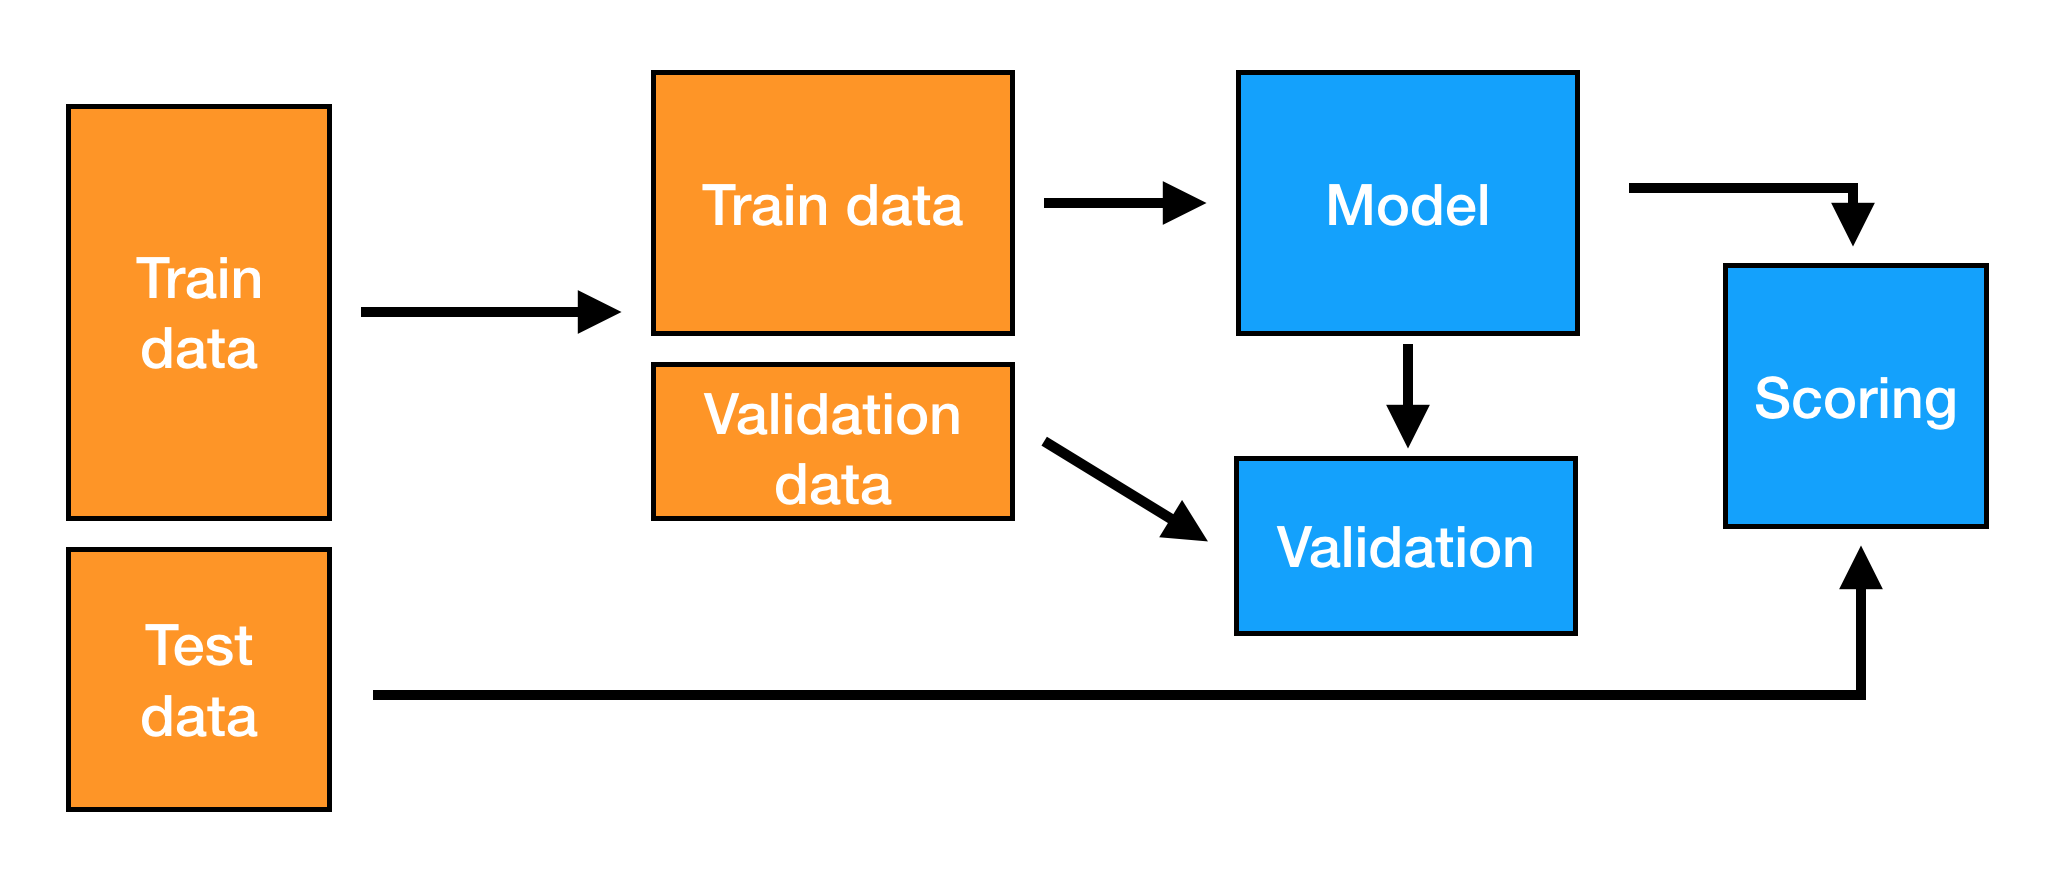
\includegraphics[width=.9\textwidth]{images/batch_learning.png}
\caption{Batch learning model (Offline learning)} \label{fig:batch}
\end{figure}

\begin{figure}[H]
\centering
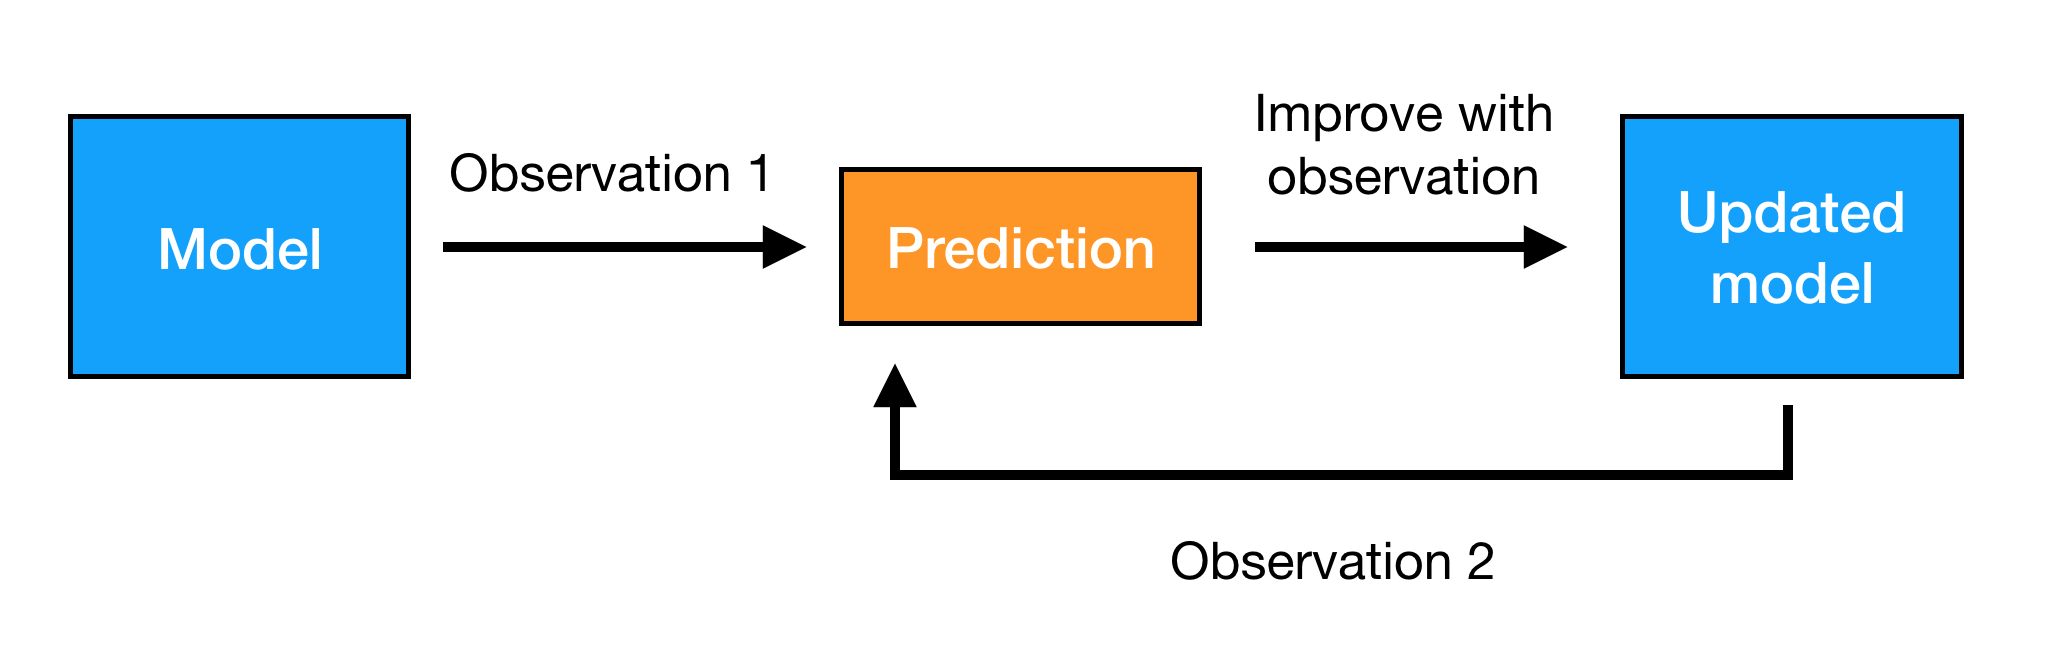
\includegraphics[width=.9\textwidth]{images/online_learning.png}
\caption{Online learning model} \label{fig:online}
\end{figure}



